%!TeX root=MemoriaTFG.tex

\chapter{Diseño e implementación del proyecto} \label{diseño_implementacion}

En este capítulo se recogen las características de diseño del proyecto, así como también su posterior implementación. A continuación se detallarán cómo son el programa principal, el agente y el entorno del problema, cómo se relacionan, y finalmente, cómo están implementados. 

\section{Diseño del proyecto}

Para poder realizar la implementación del proyecto, es necesario diseñar los elementos principales que lo conforman: el programa principal que controla la ejecución, la definición de los elementos empleados en el programa y las distintas funcionalidades que se desea que tengan.  

\subsection{Diseño del programa}

El programa principal es el elemento de control de la ejecución. Se ha diseñado de tal forma que el usuario tiene control casi al completo de todas las características de la ejecución de un experimento a partir de sus especificaciones concretas. Además, el usuario también podrá elegir de la lista de experimentos previamente realizados y podrá ver las gráficas con los resultados obtenidos. \\

Las especificaciones del usuario sobre el experimento son:
\begin{enumerate}
    \item Las \textbf{iteraciones} y los \textbf{episodios} totales del experimento.
    \item Las \textbf{dimensiones} del entorno.
    \item El \textbf{tipo de ejecución} de desea realizar, si bien un nuevo experimento o la visualización de  resultados de experimentos anteriores. 
    \item El \textbf{tipo de modelo} que se debe emplear. Los distintos tipos se explicarán en el apartado \ref{tiposModelos}.
    \item El \textbf{tipo de experimento} que se quiere llevar a cabo. Los experimentos que se pueden realizar se explicarán en el apartado \ref{tiposExperimentos}.
\end{enumerate}

El experimento puede contener varias iteraciones, con cada iteración un total de episodios concreto. Los episodios hacen referencia a la veces que el agente busca su camino hacia el objetivo. Con cada episodio, el entorno se reinicia a su estado inicial y se comienza de nuevo. Los episodios pueden llegar a una solución o no. \\

El objetivo de tener distintas iteraciones, además de entrenar la red, es para\textit{ modificar las condiciones del entorno} y \textit{observar la adaptación del agente}. Las condiciones que se modifican son las \textbf{posiciones del agente} y del \textbf{objetivo}. 

\subsubsection{Tipos de modelos} \label{tiposModelos}

Los modelos hacen referencia al modelo interno del agente que compone la red neuronal. El modelo puede ser
\begin{itemize}
    \item Un \textbf{modelo nuevo}, es decir, una red neuronal inicializada con sus pesos aleatoriamente y sin entreno previo. 
    \item Un \textbf{modelo existente}; dicho modelo ya habrá sido sometido a uno o varios experimentos, por lo que tendrá los pesos ya ajustados con unos valores determinados. 
\end{itemize}

Una vez realizado un experimento se puede guardar el modelo resultante y los resultados de dicho experimento. 


\begin{figure}[ht!]
    \centering
    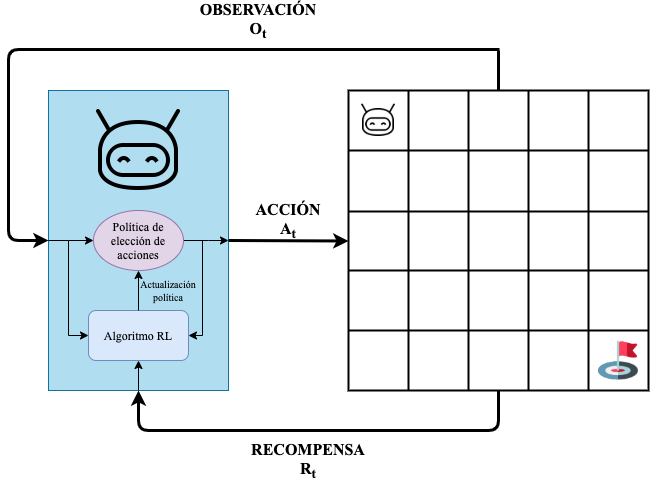
\includegraphics[scale=0.5]{cap4_diseño_implementacion/images/diagrama_RL.png}
    \caption{Ecosistema del proyecto compuesto por el entorno y el agente.}
    \label{fig:red_neuronal_simple}
\end{figure}

El problema propuesto, como bien se ha mencionado anteriormente en el capítulo \ref{introduccion}, tiene un ecosistema formado por: 
\begin{enumerate}
    \item Un \textbf{entorno} que contiene toda la información del problema: la \textbf{estructura} del espacio en el que se desarrollan las acciones, las \textbf{dimensiones} del espacio, las \textbf{acciones} que se pueden realizar, las \textbf{percepciones} observables que describen cómo va cambiando el entorno con cada acción realizada y, por último, las \textbf{recompensas} que se reciben con cada acción dependiendo del estado en el que se encuentra el entorno. 
    \item Un \textbf{agente inteligente} que debe interaccionar con el entorno con el fin de cumplir un objetivo definido. Las interacciones que puede tener con el entorno van definidas por una serie de acciones concretas. 
\end{enumerate}

En la Fig.~\ref{fig:red_neuronal_simple} se puede observar dicho ecosistema con los elementos y las interacciones posibles entre ellos. \\

A continuación se detallará el diseño de ambos elementos a alto nivel. 

\subsection{Diseño del entorno}

Para el diseño del entorno se deben tener en cuenta su \textit{estructura}, las \textit{acciones que se pueden realizar}, las \textit{percepciones} y las \textit{recompensas} que se ofrecen al agente. 

\subsubsection{Modelización del entorno} 

El entorno del problema tiene una \textbf{estructura matricial} y se muestra en la Fig.~\ref{fig:estructura_entorno}. Las dimensiones del entorno son \textbf{\textit{dinámicas}} - no hay un tamaño fijo definido sino que se permite minimizar o ampliar las dimensiones. 

\begin{figure}
    \centering
    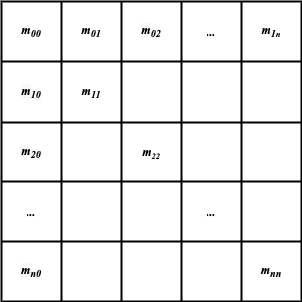
\includegraphics[scale=0.4]{cap4_diseño_implementacion/images/entorno.png}
    \caption{Estructura del entorno.}
    \label{fig:estructura_entorno}
\end{figure}

\subsubsection{Acciones permitidas}

Sea $n$ la dimensión de la matriz, $x$ el índice de las filas e $y$ el índice de las columnas de la matriz del entorno. El rango de los valores se encuentra entre de $x$ e $y$ entre $0 - (n - 1)$. Las acciones permitidas para el desplazamiento dentro de este entorno son: 
\begin{enumerate}
    \item \textbf{\textit{Arriba}}: desplazamiento de una casilla $m_{xy}$ a una casilla $m_{xy-1}$.
    \item \textbf{\textit{Abajo}}: desplazamiento de una casilla $m_{xy}$ a una casilla $m_{xy+1}$.
    \item \textbf{\textit{Derecha}}: desplazamiento de una casilla $m_{xy}$ a una casilla $m_{x+1y}$.
    \item \textbf{\textit{Izquierda}}: desplazamiento de una casilla $m{xy}$ a una casilla $m_{x-1y}$. 
\end{enumerate}
Dichas acciones se representan en la Figura \ref{fig:acciones_entorno}. \\
\begin{figure}
    \centering
    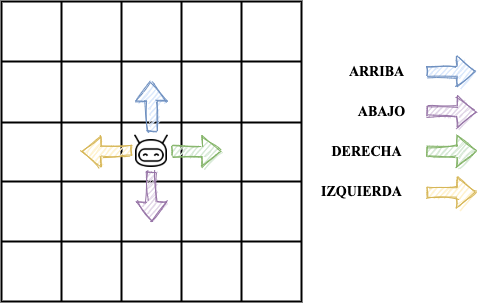
\includegraphics[scale=0.5]{cap4_diseño_implementacion/images/acciones.png}
    \caption{Acciones del entorno.}
    \label{fig:acciones_entorno}
\end{figure}

En la nomenclatura de la librería \textit{Gym}, el número total de acciones que se realizar hacer se denomina $action\_space$, es decir, espacio de acciones.

\subsubsection{Percepciones del entorno} En el entorno se conoce en cada \textbf{\textit{estado}} cuál es la \textbf{posición exacta del agente}; los estados, por lo tanto, codifican una posición de la matriz. Los estados no contemplan si se ha llegado al objetivo, sino que se comprueba con cada movimiento realizado si el nuevo estado en el que se encuentra el entorno se corresponde con la \textbf{posición del objetivo} que se debe alcanzar. \\

\begin{figure}[!h]
    \centering
    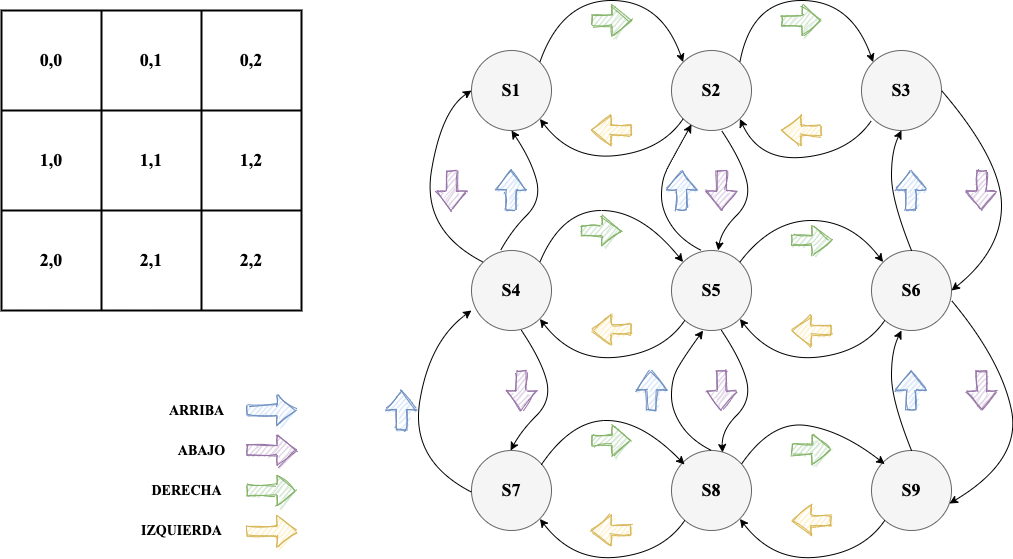
\includegraphics[scale=0.4]{cap4_diseño_implementacion/images/estados_3x3.png}
    \caption{Ejemplo de diagrama de estados de un entorno con una dimensión de 3x3.}
    \label{fig:estados_3x3}
\end{figure}

Los \textbf{estados totales} que puede tener el entorno viene determinado por sus dimensiones, y se calcula como $n^2$. Como se puede observar en la Fig.~\ref{fig:estados_3x3}, un entorno con unas dimensiones de $3x3$ tendría un \textbf{total de 9 estados diferentes}. \\

En la nomenclatura de la librería \textit{Gym}, el número total de estados en el que se puede encontrar el entorno se denomina $observation\_space$, es decir, espacio de observaciones (percepciones).

\subsubsection{Recompensas} 

Una recompensa es aquella percepción del entrono que muestra si la acción realizada anteriormente ha supuesto un avance hacia el objetivo del agente. Las recompensas son aquellas que el agente valorará para determinar si su comportamiento es eficiente y si le permite acercarse cada vez más al objetivo. \\

Existen 2 tipos de recompensas: 

\begin{enumerate}
    \item El agente deberá recibir \textbf{una recompensa positiva} siempre que haga \textbf{una acción lógica dentro del entorno} que le perimta estar más cerca del objetivo propuesto. 
    \item El agente deberá recibir \textbf{una recompensa negativa} cuando realice \textbf{una acción que le suponga estar más lejos de su objetivo}, o bien cuando realiza una acción que implique salir del rango permitido del entorno. 
\end{enumerate}


\begin{figure}
    \centering
    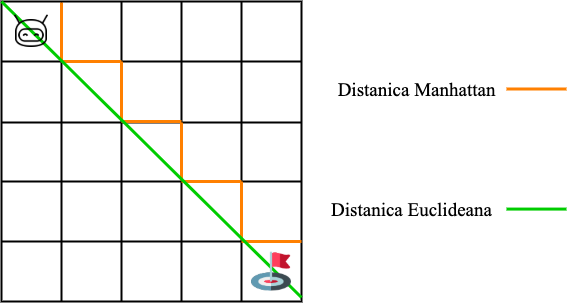
\includegraphics[scale=0.4]{cap4_diseño_implementacion/images/recompensa_distancia.png}
    \caption{Distancia de Manhattan y Euclideana en una matriz de dimensiones 5x5.}
    \label{fig:recompensa_distancia}
\end{figure}

\begin{figure}
    \centering
    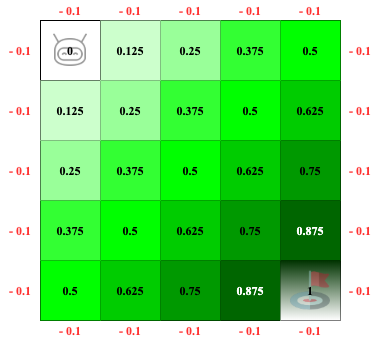
\includegraphics[scale=0.55]{cap4_diseño_implementacion/images/rewards_5x5.png}
    \caption{Recompensas del entorno de 5x5 según la distancia al objetivo. Se considera que el objetivo está en la posición (4, 4).}
    \label{fig:rewards_5x5}
\end{figure}

En el caso de las recompensas positivas, éstas se calculan teniendo en cuenta la \textbf{distancia de Manhattan} entre la posición del agente y la posición del objetivo. Se ha elegido este tipo de distancia debido a la naturaleza de la estructura del entorno (matricial) y a las acciones que se pueden realizar. \\

La recompensa se ha normalizado para tener valores entre 0 y 1, y se calcula de la siguiente forma: 

$$ d_{normalizada} = 1 - \frac{d_{Manhattan}} {d_{maxima}}$$


Cuanto más cerca esté el agente del objetivo, la recompensa recibida será mayor. Se puede observar la evolución de la recompensa en la Fig.~\ref{fig:rewards_5x5}.


\subsection{Diseño del agente} \label{diseñoAgente}

Uno de los requisitos del proyecto (véase Req.~\ref{requerimientos}) era \textbf{la necesidad de utilizar una red neuronal} para el agente. \\

En la figura \ref{fig:NN4_25_25_4} se muestra la red implementada para este problema. La dimensión y las capas de la red neuronal utilizada para la experimentación surgió tras la realización de diversas pruebas. Se optó por mantener este modelo constante a lo largo de las diferentes pruebas con el objetivo de simplificar la interpretación de los resultados.\\

El algoritmo de aprendizaje empleado para la red neuronal es el \textbf{DQN}, explicado anteriormente en el apartado \ref{dqn-learning}. 

\begin{figure}
    \centering
    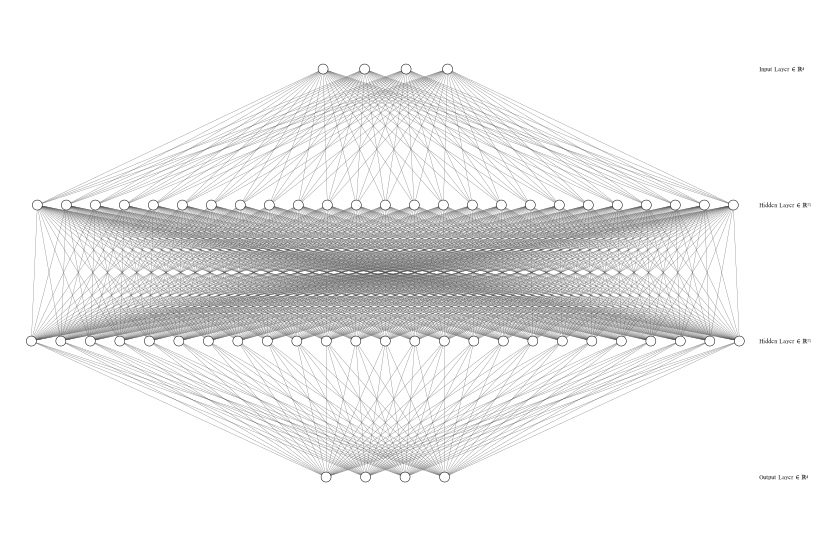
\includegraphics[scale=0.45]{cap4_diseño_implementacion/images/NN4_25_25_4.png}
    \caption{Red neuronal de 4 capas con 4, 25, 25, 4 neuronas, respectivamente.}
    \label{fig:NN4_25_25_4}
\end{figure}

\section{Implementación del proyecto}

Los detalles más significantes de la implementación se detallan a continuación. La Fig.~\ref{fig:diagrama_RL_funciones} sintetiza aquellas funciones implementadas dentro del modelo del entorno y del agente. De derecha a izquierda, tenemos:

\begin{enumerate}
    \item La implementación del entorno, en la que se muestra la estructura que lo compone y un ejemplo de transición entre estados mediante la realización de una acción por parte del agente. El entorno, una vez realizada la acción, devuelve una serie de percepciones al agente. 
    \item La implementación del agente, en la que se muestran los componentes que permiten el aprendizaje y las distintas interacciones que tiene con el entorno. Los componentes de aprendizaje son la política de acciones $\pi$, la función \texttt{replay}, la memoria de repetición $\mathbbb{D}$.
\end{enumerate}

\begin{figure}
    \centering
    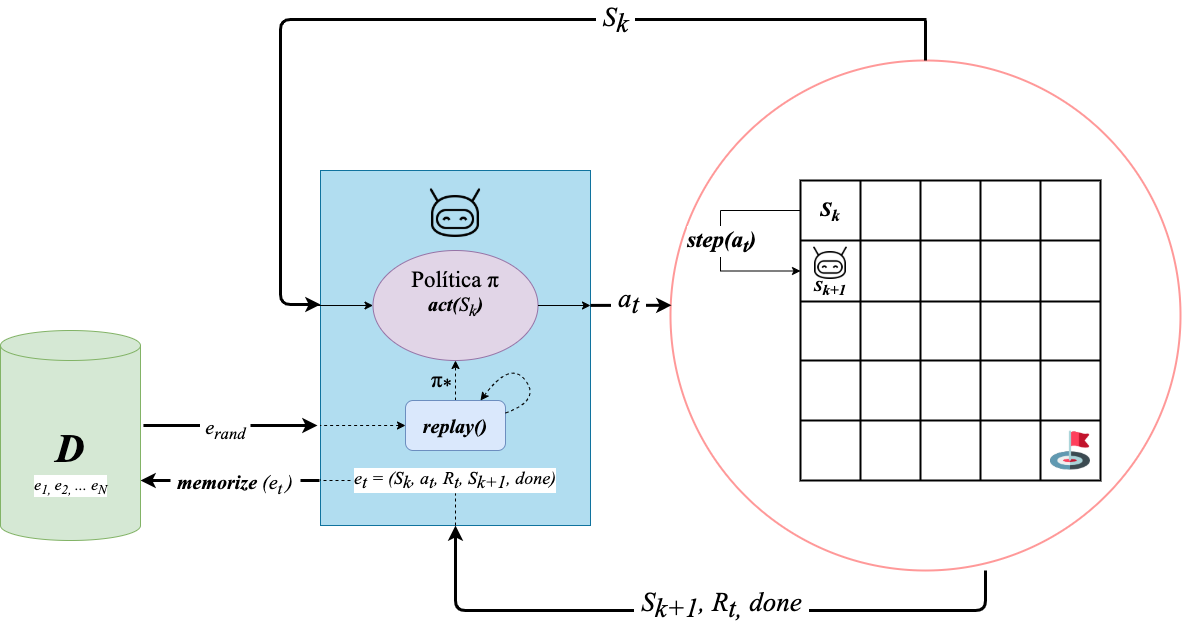
\includegraphics[scale=0.39]{cap4_diseño_implementacion/images/diagrama_RL_funciones.png}
    \caption{Implementación del ecosistema del problema.}
    \label{fig:diagrama_RL_funciones}
\end{figure}
A continuación se explicará el programa principal que se encarga de controlar la ejecución del proyecto. 

%TODO ISAAC-WAIT-SECCION
\subsection{Implementación del programa}

La implementación del programa principal se encarga de encajar todas las piezas (el agente y el entorno y sus características) y de realizar la ejecución siguiendo las especificaciones del usuario. Recordemos que el usuario puede especificar: 
\begin{enumerate}
    \item El total de iteraciones y de episodios que tendrá el experimento. 
    \item Las dimensiones del entorno.
    \item El tipo de ejecución de desea realizar.
    \item El tipo de modelo que se debe emplear. 
    \item El tipo de experimento que se quiere llevar a cabo. 
\end{enumerate}

Los métodos más importantes del programa son: 

\begin{enumerate}
    \item \texttt{run\_experiment}: Controla las iteraciones del experimento y recoge todos los resultados de cada una. Además, si es necesario, modifica las posiciones del agente o del objetivo. 
    \item \texttt{compute\_iteration}: Como el propio nombre indica, realiza una iteración con todos sus episodios. \\
    
    En cada episodio $ep$ se resetea el entorno a su estado inicial $S_0$ y se lanza el agente para que encuentre la combinación de movimientos que lleve al objetivo. Si se llega al objetivo, se actualiza el target con los Q-values actuales (tal como está explicado en el apartado \ref{dqn-learning-replay}). Cuando la memoria de repetición $D$ haya sobrepasado una cierta cantidad de experiencias $MAX\_MEMORY$ se lanzará la función de \texttt{replay} para aprender de la experiencia. \\

\subsubsection{Función \texttt{compute\_iteration}}

La función que controla la ejecución y las distinta interacciones entre el entorno y el agente es la función \texttt{compute\_iteration}, y se muestra en el Alg. ~\ref{compute_iteration}. \\

Este método se ejecuta tantas veces como iteraciones haya definido el usuario. Para cada episodio que hay en una iteración (línea ~\ref{lst:line:computeIterationLine1}), se resetea el estado del entorno a su estado inicial $S_0$ (línea ~\ref{lst:line:computeIterationLine2}). A continuación se realiza la búsqueda de la secuencia de acciones que lleven al objetivo. El número máximo de acciones que puede realizar el agente viene definido por la variable $steps$. Las acciones se calculan teniendo en cuenta el estado actual del entorno (línea~\ref{lst:line:computeIterationLine4}); una vez elegida la acción el agente se mueve dentro del entorno (línea ~\ref{lst:line:computeIterationLine5}) y guarda la experiencia resultante en la memoria de repetición (línea ~\ref{lst:line:computeIterationLine6}). El estado del entorno se actualiza y, en caso de que se haya alcanzado el objetivo, se guarda el modelo actual como el óptimo (línea ~\ref{lst:line:computeIterationLine9}) y se termina la ejecución del episodio. Si el tamaño de la memoria de repetición ha superado la cantidad $MAX\_MEMORY$, se realiza el aprendizaje empleando la función \texttt{replay} (línea ~\ref{lst:line:computeIterationLine12}), explicado en el Alg. ~\ref{replayAlgorithm}. \\
\begin{algorithm}[H]
\SetAlgoLined
\SetKwInOut{Input}{input}
\SetKwInOut{Output}{output}
\SetKw{KwIn}{in}
\SetKw{KwBreak}{break}
\SetKw{KwNot}{not}
\SetKwData{Episodes}{$episodes$}
\SetKwData{Episode}{$ep$}
\SetKwData{Actions}{$actions$}
\SetKwData{Step}{$t$}
\SetKwData{Steps}{$steps$}
\SetKwData{BatchSize}{$batch\_size$}
\SetKwData{Done}{$done$}
\SetKwData{Action}{$a_t$}
\SetKwData{MaxMem}{$MAX\_MEMORY$}
\SetKwData{State}{$S_k$}
\SetKwData{InitialState}{$S_0$}
\SetKwData{NextState}{$S_{k+1}$}
\SetKwData{Env}{$env$}
\SetKwData{Agent}{$agent$}
\SetKwData{Reward}{$R_t$}
\SetKwData{Memory}{$D$}
\SetKwData{IterationResults}{$iteration\_results$}
\SetKwData{EpsSolved}{$episodes\_solved$}
\SetKwData{StepsTaken}{$steps\_taken$}
\SetKwData{EpisodeRewards}{$episode\_rewards$}
\SetKwData{EpisodeReward}{$episode\_reward$}
\SetKwFunction{Append}{append}
\SetKwFunction{ComputeIteration}{$compute\_iteration$}
\SetKwFunction{Act}{act}
\SetKwFunction{StepAction}{step}
\SetKwFunction{Memorize}{memorize}
\SetKwFunction{Len}{len}
\SetKwFunction{UpdateTargetModel}{$update\_target\_model$}
\SetKwFunction{Replay}{replay}
\Input{$episodes$}
\BlankLine
\For{\Episode \KwIn \Episodes}{\label{lst:line:computeIterationLine1}
    \State $\leftarrow$ \InitialState\;\label{lst:line:computeIterationLine2}
    \For{\Step \KwIn \Steps}{
        \Action $\leftarrow$ \Agent.\Act{\State}\;\label{lst:line:computeIterationLine4}
        \NextState, \Reward, \Done $\leftarrow$ \Env.\StepAction{\Action}\;\label{lst:line:computeIterationLine5}
        \Agent.\Memorize{\State, \Action, \Reward, \NextState, \Done}\;\label{lst:line:computeIterationLine6}
        \State $\leftarrow$ \NextState\;
        \uIf{\Done}{
            \Agent.\UpdateTargetModel{}\;\label{lst:line:computeIterationLine9}
            \KwBreak\;
        }
        \uIf{\Len{\Memory} > \MaxMem}{
            \Agent.\Replay{\BatchSize}\;\label{lst:line:computeIterationLine12}
        }  
    }
}
 \caption{Función \texttt{compute\_iteration}} \label{compute_iteration}
\end{algorithm}
\end{enumerate}

\subsection{Implementación del entorno}

La implementación del entorno se ha realizado mediante la clase básica de la librería \textit{Gym}: \texttt{Env} \cite{gymCore}. Las operaciones que define son:

\begin{enumerate}
    \item \texttt{\textbf{step}}: Aplica una acción $a$ al entorno. Dicha acción provoca un cambio de estado en el entorno, y éste devuelve como resultados de esta función
    \begin{enumerate}
        \item \texttt{\textit{observation}}: El nuevo estado de entorno.
        \item \texttt{\textit{reward}}: La recompensa obtenida a raíz de la realización de la acción $a$.
        \item \texttt{\textit{done}}: Determina si el episodio ha acabado, es decir, si se ha llegado al objetivo. 
        \item \texttt{\textit{info}}: Sirve para imprimir información auxiliar que puede ser útil para \textit{debuggear}. 
    \end{enumerate}
    \item \texttt{\textbf{reset}}: Resetea el entorno a su estado inicial y retorna dicho estado. 
    \item \texttt{\textbf{render}}: Visualiza el entorno. Existen varios modos de visualización: $human$, $rgb\_array$ y $ansi$.
    \item \texttt{\textbf{close}}: Finaliza el programa y limpiar
    la memoria. En caso de que no se implemente, el propio entorno $"$se cierra$"$ cuando el programa se cierra. 
    \item \texttt{\textbf{seed}}: Fija la \textit{semilla} de generación pseudoaleatoria de número que controlan las interacciones con el agente. 
\end{enumerate}

De estos 5 métodos \textbf{se han sobrescrito 2, \textit{\texttt{step}} y \textit{\texttt{reset}}}. \\

\subsubsection{Función \texttt{step}}

La función \texttt{step}, como ya se ha mencionado, corresponde a la realización de la acción ($a_t$) dentro del entorno. Para poder aplicar la acción $a_t$ se debe primero eliminar el agente de la posición $agent\_pos$ en la que estaba antes de realizar la acción (línea ~\ref{lst:line:stepLine1} del Alg. ~\ref{stepAlgorithm}). Una vez hecho esto, se calcula su nueva posición $next\_agent\_pos$ (línea ~\ref{lst:line:stepLine2}) teniendo en cuenta la acción elegida $a_t$ y se actualiza el entorno con la nueva posición (línea ~\ref{lst:line:stepLine3}). Por último, se calcula la recompensa total obtenida $R_t$ (línea ~\ref{lst:line:stepLine5}) tras realizar este movimiento, y se comprueba si el agente ya ha llegado a la posición del objetivo (línea ~\ref{lst:line:stepLine6}). La función GetReward se describe en el Alg. ~\ref{GetReward}. 

\begin{algorithm}[H]
\SetAlgoLined
\SetKwInOut{Input}{input}
\SetKwInOut{Output}{output}
\SetKwData{NextAgentPos}{$next\_agent\_pos$}
\SetKwData{Penalty}{$use\_penalty$}
\SetKwData{Reward}{$R_t$}
\SetKwData{Done}{$done$}
\SetKwData{AgentPos}{$agent\_pos$}
\SetKwData{Action}{$a_t$}
\SetKwData{GoalPosition}{$goal\_position$}
\SetKwData{State}{$S_k$}
\SetKwData{NextState}{$S_{k+1}$}
\SetKwFunction{GetReward}{GetReward}
\SetKwFunction{GetNextPosition}{GetNextPosition}
\Input{$a_t$}
\Output{$S_{k+1}, R_t, done$}
\BlankLine
\State[\AgentPos] $\leftarrow$ $0$\;  \label{lst:line:stepLine1} 
\NextAgentPos, \Penalty $\leftarrow$ \GetNextPosition{\Action,\AgentPos}\;\label{lst:line:stepLine2} 
\State[\NextAgentPos] $\leftarrow$ $1$\; \label{lst:line:stepLine3} 
\NextState $\leftarrow$ \State\;
\Reward $\leftarrow$ \GetReward{\NextAgentPos, \Penalty}\;\label{lst:line:stepLine5} 
\Done $\leftarrow$ \NextAgentPos $\equiv$ \GoalPosition\; \label{lst:line:stepLine6}
return \NextState, \Reward, \Done\;
 \caption{Función \textit{\texttt{step}}} \label{stepAlgorithm}
\end{algorithm} 

\subsubsection{Función \texttt{GetReward}}

La función \texttt{GetReward}, mostrada en el Alg.~\ref{GetReward}, sirve para calcular la recompensa obtenida después de un movimiento realizado. Para calcular la recompensa $R_t$ se necesita la posición actual de agente $agent\_pos$; además, se tiene una variable $use\_penalty$ que indica si el movimiento realizado previamente ha causado que el agente salga del rango del entorno: en caso afirmativo, en lugar de recompensa el agente recibe una penalización con valor de -0.1 (línea ~\ref{lst:line:getRewardLine2}). Si de lo contrario el movimiento era válido, se calcula la distancia Manhattan (línea ~\ref{lst:line:getRewardLine4}) de la posición actual del agente hasta la posición del objetivo. La distancia normalizada (línea ~\ref{lst:line:getRewardLine5}) se corresponde a la recompensa que se devuelve (línea ~\ref{lst:line:getRewardLine7}). \\

\begin{algorithm}[H]
\SetAlgoLined
\SetKwInOut{Input}{input}
\SetKwInOut{Output}{output}
\SetKwData{Reward}{$R_t$}
\SetKwData{Penalty}{$use\_penalty$}
\SetKwData{AgentPos}{$agent\_pos$}
\SetKwData{Distance}{$d_{manhattan}$}
\SetKwData{MaxDistance}{$d_{maxima}$}
\SetKwData{GoalPosition}{$goal\_position$}
\SetKwFunction{Cityblock}{cityblock}
\Input{$agent\_pos$, $use\_penalty$}
\Output{$R_t$}
\BlankLine
\eIf{\Penalty}{
   \Reward $\leftarrow$ $-0.1$ \; \label{lst:line:getRewardLine2}
   }{
\Distance $\leftarrow$ \Cityblock{\AgentPos, \GoalPosition} \;\label{lst:line:getRewardLine4}
\Reward $\leftarrow$ 1 - (\Distance / \MaxDistance) \;\label{lst:line:getRewardLine5}
}
return \Reward \;\label{lst:line:getRewardLine7}
 \caption{Función \textit{\texttt{GetReward}}} \label{GetReward}
\end{algorithm}

\subsection{Implementación del agente}

El agente se ha implementado utilizando el modelo \texttt{Sequential} de la librería \texttt{Keras}. Tal como se explica en la documentación oficial de Keras \cite{kerasSequential}, este modelo \textit{se utiliza para una simple agrupación de capas donde cada capa tiene exactamente un tensor de entrada y un tensor de salida}. \\

La arquitectura de la red neuronal empleada se compone por 4 capas de 4, 25, 25, 4 neuronas respectivamente, y se muestra en la Fig. ~\ref{fig:NN4_25_25_4}. Las distintas capas tienen como función de activación: 

\begin{itemize}
    \item \textbf{linear}: Las primeras 3 capas de la red. La salida de las neuronas se calculan teniendo en cuenta la suma de los valores de las entradas multiplicadas por los pesos de cada una. 
    \item \textbf{softmax}: La última capa, ya que es interesante ver los resultados de la red como un porcentaje para que la interpretación sea más intuitiva. Tal como se explica en \cite{activationFunctionTypes}, esta función trata con múltiples clases y es capaz de normalizar la salida de la red para cada clase para que tengan valores entre 0 y 1. Estos valores, además, representan las probabilidades que tiene cada acción de ser elegida.
\end{itemize}

\begin{figure}
    \centering
    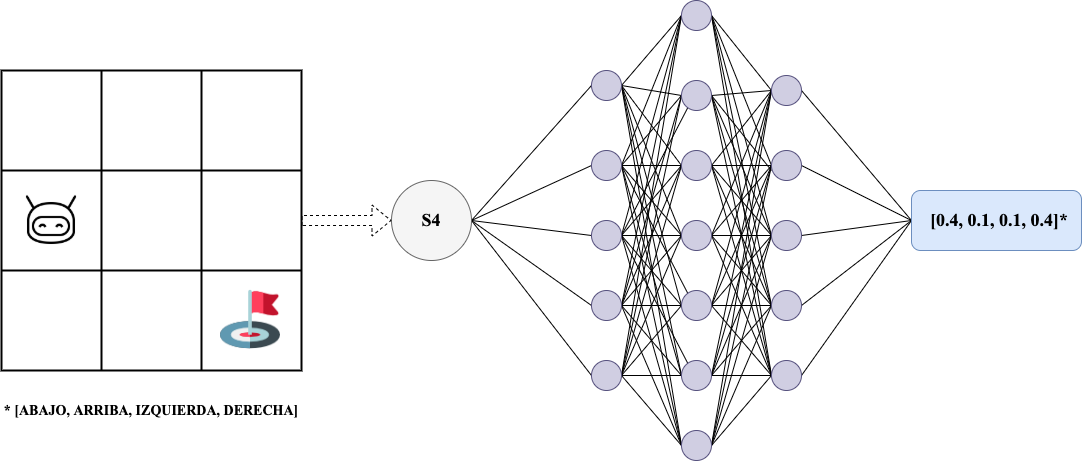
\includegraphics[scale=0.4]{cap4_diseño_implementacion/images/nn_input_output.png}
    \caption{Entrada y salida del agente.}
    \label{fig:nn_input_output}
\end{figure}

En este caso, la entrada del modelo es el \textbf{estado del entorno}, y la salida es una \textbf{lista de predicciones} que se corresponde con las \textbf{probabilidades de cada acción} de realizarse en esas condiciones concretas. \\

Un ejemplo de ello se muestra en la Fig.~\ref{fig:nn_input_output}, donde un agente se encuentra en la posición (1, 0) de la matriz. Dicha posición se corresponde con el estado $S_4$ y a partir de la evaluación de la red neuronal interna del agente se le ha asociado a este estado una probabilidad por cada acción que se puede realizar, en concreto: 0.4 si se mueve hacia abajo, 0.1 si se mueve hacia arriba, 0.1 si se mueve a la izquierda y 0.4 si se mueve a la derecha. \\
   
A continuación se explicarán las funcionalidades del agente implementadas. 

\subsubsection{Función \texttt{act}}

Función que determina \textbf{qué acción $a_t$ es la mejor para tomar a continuación dado un estado $S_k$} en concreto del entorno. Para ello, la red neuronal debe predecir para cada acción la probabilidad $\mathbb{P}_{A}$ de ser elegida; en base a dicha predicción, se escoge la acción con mayor probabilidad de ocurrir y se retorna. \\

\subsubsection{Función \texttt{memorize}}

Función que sirve para \textbf{guardar} en la \textit{memoria de repetición} del agente $D$ \textbf{la experiencia obtenida} $e_t$ compuesta por el estado $S_k$, acción $a_t$, siguiente estado $S_{k+1}$ y si ha llegado al objetivo. Es el proceso de aprendizaje, y mediante este método es como se \textit{construye la experiencia}. 

\subsubsection{Función \texttt{replay}}

Esta función es un tipo de técnica denominada \textbf{\textit{repetición de experiencia}} que se utiliza durante el periodo de entreno de la red. Tal como se explica en \cite{stack2017expreplay, deeplizardReplay}, para cada instante de tiempo $t$ de entreno se guarda una tupla que contiene la experiencia obtenida $e_t = (S_k, a_t, S_{k + 1}, R_t)$. Todas las tuplas de la experiencia del agente se guardan en la \textit{memoria de repetición} $D$, y será de éste conjunto de datos de dónde se tomarán muestras aleatorias para entrenar a la red. \\

En el Alg. ~\ref{replayAlgorithm} se muestra la implementación de la función \texttt{replay}. Inicialmente se comienza seleccionando una cantidad de muestras aleatorias de la memoria de repetición (línea ~\ref{lst:line:replayLine2}) que servirán como muestras de entreno para el agente. Si la red sólo aprendiese de las muestras consecutivas de experiencia que suceden de manera secuencial en el entorno, las muestras estarían altamente correlacionadas y llevaría a un aprendizaje ineficiente. El hecho de seleccionar muestras aleatorias rompe esta correlación. \\

Para cada muestra en concreto se obtiene la recompensa $R_t$ (línea ~\ref{lst:line:replayLine3}) y, en caso de que dicha experiencia no sea una en la que el agente haya alcanzado su objetivo, se recalcula la recompensa (línea ~\ref{lst:line:replayLine5}) aplicándole el descuento $\gamma$ para que refleje que no se ha conseguido alcanzar el objetivo. A continuación, se obtiene la lista de predicciones $target$ para el estado $S_k$ (línea ~\ref{lst:line:replayLine6}) y se le asigna la recompensa calculada $R_t$ al elemento de la lista correspondiente a la acción $a_t$ (línea ~\ref{lst:line:replayLine7}). Finalmente, se entrena la red dados los estados y las listas de predicciones obtenidas previamente (línea ~\ref{lst:line:replayLine11}) y se devuelve el error total obtenido.  \\
\begin{algorithm}[H]
\SetAlgoLined
\SetKwInOut{Input}{input}
\SetKwInOut{Output}{output}
\SetKwData{States}{$states$}
\SetKwData{Targets}{$targets$}
\SetKwData{Reward}{$R_t$}
\SetKwData{History}{$history$}
\SetKwData{ValueReward}{$value\_reward$}
\SetKwData{Memory}{$memory$}
\SetKwData{Random}{$random$}
\SetKwData{Loss}{$loss$}
\SetKwData{Minibatch}{$minibatch$}
\SetKwData{Batchsize}{$batch\_size$}
\SetKwData{Gamma}{$\gamma$}
\SetKwData{Target}{$target$}
\SetKwData{Model}{$model$}
\SetKw{KwIn}{in}
\SetKwData{Done}{$done$}
\SetKwData{Action}{$a_t$}
\SetKwData{State}{$S_k$}
\SetKwData{NextState}{$S_{k+1}$}
\SetKwFunction{Append}{append}
\SetKwFunction{Predict}{predict}
\SetKwFunction{Fit}{fit}
\SetKwFunction{Sample}{sample}
\Input{$batch\_size$}
\Output{$loss$}
\BlankLine
\Minibatch $\leftarrow$ \Random.\Sample{\Memory, \Batchsize}\;\label{lst:line:replayLine2}
\For{\State, \Action, \Reward, \NextState, \Done \KwIn \Minibatch}{\label{lst:line:replayLine2}
    \ValueReward $\leftarrow$ \Reward\;\label{lst:line:replayLine3}
    \uIf {$not$ \Done}{
        \ValueReward $\leftarrow$ (\ValueReward + \Gamma * max(\Model.\Predict{\NextState}))\;\label{lst:line:replayLine5}
    }
    \Target $\leftarrow$ \Model.\Predict{\State}\;\label{lst:line:replayLine6}
    \Target[\Action] = \ValueReward\;\label{lst:line:replayLine7}
    \States.\Append{\State}\;
    \Targets.\Append{\Target}\;
}
\History $\leftarrow$ \Model.\Fit{\States, \Targets}\;\label{lst:line:replayLine11}
\Loss $\leftarrow$ \History[$'loss'$]\;
return \Loss\;
 \caption{Función replay} \label{replayAlgorithm}
\end{algorithm}

\subsubsection{Función \texttt{predict}}

Mediante éste método se invoca al \texttt{predict} correspondiente a la red neuronal (implementado por la clase \texttt{Sequential} de Keras) y se obtienen las predicciones para las acciones posibles. Es necesario conocer el estado actual $S_k$ del entorno para poder realizar la predicción. \\



En este capítulo se ha visto en detalle el diseño y la implementación del proyecto. Se ha visto la estructura del programa principal, así como también el flujo de la interacción entre el entorno y el agente. Para el entorno del problema se han explicado las 2 funciones fundamentales que le permite interactuar con el agente: las funciones \texttt{step} y \texttt{GetReward}. Para el agente se han explicado las funciones que sirven para realizar el aprendizaje, en concreto las funciones \texttt{memorize}, \texttt{replay} y \texttt{predict}, y también la función \texttt{act} que le permite al agente moverse por el entorno. \\

El flujo del programa y de las interacciones entre los elementos es el siguiente: \\
\renewcommand{\labelenumii}{\arabic{enumi}.\arabic{enumii}.}
\renewcommand{\labelenumiii}{\arabic{enumi}.\arabic{enumii}.\arabic{enumiii}.}
\renewcommand{\labelenumiv}{\arabic{enumi}.\arabic{enumii}.\arabic{enumiii}.\arabic{enumiv}.}
\begin{enumerate}
    \item Para \textbf{cada iteración}:
    \begin{enumerate}
        \item Para \textbf{cada episodio} de la iteración: 
        \begin{enumerate}
            \item \textbf{Resetear} el entorno a su estado inicial.
            \item Mientras el número total de acciones realizadas \textbf{no supere} el máximo permitido:
            \begin{enumerate}
                \item \textbf{Encontrar la acción} con más probabilidades de ejecutarse en el estado actual. 
                \item \textbf{Realizar el movimiento} en el entorno. Esto implica: 
                \begin{itemize}
                    \item Eliminar al agente de la posición actual del entorno. 
                    \item \textbf{Calcular la nueva posición} dentro del entorno dado el movimiento realizado.
                    \item \textbf{Actualizar entorno} con la nueva posición del agente. 
                    \item Calcular la \textbf{recompensa} total obtenida. La recompensa se calcula empleando la \textit{distancia de Manhattan} y, además, está normalizada entre los valores 0 y 1. Las recompensas también pueden ser negativas cuando se ha realizado un movimiento no válido, y en este caso tendrá el valor de -0.1.
                    \item Comprobar si \textbf{la nueva posición} del agente es \textbf{la misma que la posición del objetivo}. En caso afirmativo, es que se ha alcanzado el objetivo. 
                \end{itemize}
                \item \textbf{Guardar la experiencia} realizada compuesta por el estado actual, la acción realizada, el siguiente estado tras realizar la acción y la recompensa obtenida a raíz del movimiento en memoria. 
                \item Si se ha alcanzado el objetivo, \textbf{guardar la red} interna del agente como la red óptima y saltar al paso 1.1.1.
                \item Por lo contrario, se comprueba si la memoria ya tiene suficientes experiencias acumuladas y en caso afirmativo \textbf{se entrena la red} empleado muestras de experiencias de la memoria. 
            \end{enumerate}
        \end{enumerate}
    \end{enumerate}
\end{enumerate}
El código completo del proyecto se puede encontrar en este repositorio \cite{git}.\\